\documentclass{article}

\usepackage[final, nonatbib]{neurips_2024}

\usepackage[utf8]{inputenc} % allow utf-8 input
\usepackage[T1]{fontenc}    % use 8-bit T1 fonts
%\usepackage{hyperref}       % hyperlinks
%\usepackage{url}            % simple URL typesetting
\usepackage{booktabs}       % professional-quality tables
\usepackage{amsfonts}       % blackboard math symbols
\usepackage{nicefrac}       % compact symbols for 1/2, etc.
\usepackage{microtype}      % microtypography

\usepackage[table,xcdraw]{xcolor} % Add this package for row coloring

\usepackage{url}
\def\UrlBreaks{\do\/\do-}
\usepackage{breakurl}
\usepackage[breaklinks]{hyperref}

\usepackage{amsmath}
\usepackage{graphicx}
\usepackage{threeparttable}
\usepackage{wrapfig}
\usepackage[normalem]{ulem} 
\useunder{\uline}{\ul}{}
\usepackage{placeins}
\usepackage{tikz}
\usetikzlibrary{shapes, arrows.meta, positioning}

\tikzset{
    % Using simpler styles to match the input flowchart's appearance
    process/.style = {rectangle, minimum width=3cm, minimum height=1cm, text centered, draw, text width=3.5cm, align=center, fill=orange!30}, % Adjusted text width
    decision/.style = {diamond, aspect=1.5, minimum width=3cm, minimum height=1cm, text centered, draw, text width=3cm, align=center,  fill=green!30}, % Adjusted text width and aspect ratio
    arrow/.style = {thick,->,>=Stealth}
}

% \usepackage{showframe} to debug float placements visually:

\title{Tokens with Meaning: A Hybrid Tokenization Approach for NLP}

\author{
M. Ali Bayram$^1$, Ali Arda Fincan$^2$, Ahmet Semih Gümüş$^2$, Sercan Karakaş$^3$, \\
Banu Diri$^1$, Savaş Yıldırım$^4$, Demircan Çelik$^2$\\
$^1$Yıldız Technical University, $^2$Yeditepe University, $^3$University of Chicago, \\
$^4$Istanbul Bilgi University \\
\texttt{malibayram20@gmail.com}
}

\begin{document}
\maketitle

\begin{abstract}
Tokenization plays a pivotal role in natural language processing (NLP), shaping how textual data is segmented, interpreted, and processed by language models. Despite the success of subword-based tokenization techniques such as Byte Pair Encoding (BPE) and WordPiece, these methods often fall short in morphologically rich and agglutinative languages due to their reliance on statistical frequency rather than linguistic structure. This paper introduces a linguistically informed hybrid tokenization framework that integrates rule-based morphological analysis with statistical subword segmentation to address these limitations. The proposed approach leverages phonological normalization, root-affix dictionaries, and a novel tokenization algorithm that balances morpheme preservation with vocabulary efficiency. It assigns shared identifiers to phonologically variant affixes (e.g., \textit{-ler} and \textit{-lar}) and phonologically altered root forms (e.g., \textit{kitap} vs.\ \textit{kitabı}), significantly reducing redundancy while maintaining semantic integrity. The framework also incorporates special tokens for whitespace and orthographic case, including an \texttt{<uppercase>} token to prevent vocabulary inflation from capitalization. Byte Pair Encoding is integrated to support out-of-vocabulary coverage without compromising morphological coherence. Evaluation on the TR-MMLU benchmark—a large-scale, Turkish-specific NLP benchmark—demonstrates that the proposed tokenizer achieves the highest Turkish Token Percentage (90.29\%) and Pure Token Percentage (85.8\%) among all tested models. Comparative analysis against widely used tokenizers from models such as LLaMA, Gemma, and OpenAI's GPT reveals that the proposed method yields more linguistically meaningful and semantically coherent tokens. A qualitative case study further illustrates improved morpheme segmentation and interpretability in complex Turkish sentences. Although the implementation focuses on Turkish, the underlying methodology is language-independent and adaptable to other languages. This work contributes to ongoing efforts to improve tokenizer design through linguistic alignment, offering a practical and extensible solution for enhancing both interpretability and performance in multilingual NLP systems.

\textbf{Keywords:} Tokenization, Morphologically Rich Languages, Morphological Segmentation, Byte Pair Encoding, Turkish NLP, Linguistic Integrity, Low-Resource Languages
\end{abstract}

\section{Introduction}

Tokenization, the process of segmenting text into smaller linguistic units called tokens, is a foundational step in Natural Language Processing (NLP). It has a direct impact on vocabulary construction, model efficiency, semantic interpretation, and the overall performance of downstream tasks such as question answering, sentiment analysis, and machine translation\cite{liu_roberta_2019}. While traditional tokenization techniques—such as whitespace or rule-based segmentation—have been commonly used in early NLP systems, they fall short in modeling the complex morphological phenomena of many languages, particularly those that exhibit agglutination, inflectional variation, and phonological alternation.

Subword-based tokenization methods like Byte Pair Encoding (BPE) \cite{sennrich_neural_2016}, WordPiece \cite{schuster_japanese_2012}, and Unigram \cite{kudo_sentencepiece_2018} have become the de facto standard in transformer-based language models such as BERT \cite{devlin_bert_2019} and GPT \cite{radford_language_2019}. These methods address the out-of-vocabulary (OOV) problem by segmenting rare words into frequently occurring subword units, thereby balancing vocabulary size and generalization. However, despite their computational strengths, these frequency-based methods often disregard the linguistic structure of words. As a result, morphologically rich languages such as Turkish, Finnish, and Hungarian are frequently segmented in ways that violate morphemic boundaries, reducing semantic coherence and interpretability \cite{baykara_abstractive_2022, toraman_impact_2023}.

Agglutinative languages like Turkish pose specific challenges for tokenization. Words are formed by appending multiple affixes to a root, producing an expansive set of surface forms that differ only in morphological features. Phonological processes such as vowel harmony and consonant alternation further increase the diversity of surface realizations. For instance, plural suffixes like \textit{-lAr} or ablative markers like \textit{-dAn}, \textit{-tAn}, functionally represent the same morphemes but differ based on the phonological context. Similarly, root alternations like \textit{kitap}~$\rightarrow$~\textit{kitab} \textit{(book)} and \textit{göğüs}~$\rightarrow$~\textit{göğs} \textit{(chest)} are common in Turkish. Frequency-based subword models fail to account for such variation, resulting in redundant and inconsistent tokenization \cite{bayram_tokenization_2025}.

Tokenization approaches that ignore these morphological and phonological nuances lead to increased vocabulary size, fragmented representation of morphosyntactic units, and reduced performance in syntactically dependent tasks. Recent benchmark studies, including TR-MMLU \cite{bayram_setting_2025} and a cross-model tokenizer evaluation \cite{bayram_tokenization_2025}, have shown that metrics such as Turkish Token Percentage (TR~\%) and Pure Token Percentage (Pure~\%) strongly correlate with downstream model performance. These findings underscore the necessity of tokenization strategies that align with linguistic structures.

Token purity plays a critical role in the effectiveness of large language models, particularly when applied to morphologically complex languages like Turkish. Since LLMs are fundamentally statistical pattern learners, the quality and clarity of those patterns directly influence their ability to generalize, reason, and generate coherent outputs. Pure tokens—those that cleanly align with complete morphemes such as roots or affixes—provide semantically and syntactically consistent input signals. This allows models to recognize grammatical structures, identify morphological relationships, and transfer learned behavior across different word forms (e.g., \textit{kitap}, \textit{kitabı}, \textit{kitaplık}). In contrast, impure tokens—subword units that contain partial or blended morphemes—introduce ambiguity into the token stream. Such noise disrupts the alignment between token boundaries and linguistic meaning, hindering the model’s ability to learn reliable representations.

Empirical studies have shown that morphologically aware tokenization can significantly improve model performance, generalization, and interpretability. Hofmann et al.~\cite{hofmann_superbizarre_2021} demonstrated that transformer models with derivationally informed vocabularies perform better at interpreting complex word forms, even in English, a language with relatively mild morphological variation. Similarly, Jabbar~\cite{jabbar_morphpiece_2024} introduced MorphPiece, a tokenizer that segments text based on morphemes before applying subword encoding. A GPT-style model trained with this tokenizer achieved superior performance across multiple NLP benchmarks—including language modeling, zero-shot GLUE, and text embedding tasks—despite using only half the training iterations of its BPE-based counterpart. These findings provide strong evidence that token purity, grounded in morphological structure, enhances learning efficiency and leads to more transparent and generalizable language models.

The importance of token purity is analogous to segmentation practices in other machine learning domains. In computer vision, models such as capsule networks \cite{sabour_dynamic_2017} and object-centric architectures like Slot Attention \cite{locatello_slot_2020} show that performance and generalization improve when visual scenes are decomposed into discrete, meaningful entities rather than treated as undifferentiated pixel grids. Capsule networks, for example, represent objects as holistic capsules rather than scattered features, enabling more accurate recognition in complex visual settings. Similarly, Slot Attention learns to bind visual input to abstract object representations, facilitating compositional reasoning and generalization across novel configurations. The same principle applies to language modeling: when token boundaries reflect linguistic structure, the model receives clearer and more interpretable signals. Token purity is thus not merely a linguistic preference—it is a structural requirement for training high-performing, semantically aware language models. This perspective motivates our use of Pure~\% as a central evaluation metric in this study.

In response to these limitations, this paper introduces a linguistically informed, language-independent tokenization framework that integrates rule-based morphological segmentation with statistical subword modeling. The approach includes several key innovations:

First, phonological normalization is applied so that surface variants of the same morpheme are assigned a unified identifier. This includes mapping affixes with phonological variation triggered by the vowel harmony (e.g., \textit{-dAn}, \textit{-tAn} \textit{(from)}) and roots with final devoicing (e.g., \textit{kitap} and \textit{kitab} \textit{(book)}) to shared token IDs. Second, a special token (\texttt{<uppercase>}) is used to encode orthographic case distinctions, enabling models to differentiate capitalized tokens without duplicating them in the vocabulary. Third, formatting characters such as space, newline, and tab are explicitly tokenized, preserving the structural integrity of the original text for downstream tasks involving structured documents or layout-sensitive processing. Fourth, a hybrid tokenization algorithm is developed, combining dictionary-based morphological analysis with Byte Pair Encoding. While morphological segmentation ensures alignment with linguistic units, BPE provides fallback coverage for unknown words, maintaining efficiency and scalability in large corpora.

The proposed tokenizer is evaluated on the TR-MMLU benchmark to test the hypothesis that incorporating linguistic structures—particularly morphological segmentation and phonological normalization—into tokenization can significantly enhance semantic alignment and efficiency in morphologically rich languages. This hypothesis is grounded in prior empirical evidence that linguistic alignment metrics such as Turkish Token Percentage (TR~\%) and Pure Token Percentage (Pure~\%) are correlated with downstream performance on MMLU-style benchmarks \cite{bayram_tokenization_2025}. Motivated by these findings, this study aims to develop a tokenization strategy that aligns closely with Turkish morphosyntactic structures, minimizes redundancy, and improves interpretability. Empirical results validate this objective: the tokenizer achieved 90.29\% TR~\% and 85.80\% Pure~\%—the highest among all evaluated models—outperforming widely used tokenizers such as those from LLaMA, Gemma, and Qwen. These results demonstrate that tokenizers designed with linguistic integrity in mind can yield tokens that are both semantically meaningful and syntactically coherent, without relying on large vocabularies or excessive computational overhead. While the implementation is tailored to Turkish, the underlying methodology is designed to generalize across other languages.

\section{Related Work}
\label{sec:related_work}

Tokenization is a fundamental step in NLP, significantly impacting model performance, memory efficiency, and downstream task effectiveness. Tokenization strategies range from character-level segmentation to subword-based methods such as Byte Pair Encoding (BPE) \cite{sennrich_neural_2016}, WordPiece \cite{schuster_japanese_2012}, and Unigram \cite{kudo_subword_2018}. The choice of tokenization directly influences the ability of models to capture syntactic, semantic, and morphological structures, especially in morphologically rich languages like Turkish, Finnish, and Hungarian \cite{baykara_abstractive_2022, toraman_impact_2023}.

Recent research has explored alternative tokenization strategies tailored to morphologically rich languages. The morphological tokenizer introduced by \cite{toraman_impact_2023} outperformed conventional subword tokenization techniques, recovering 97\% of the performance of larger BERT-based models while reducing model size by a factor of three. Additionally, tokenization granularity has been extensively examined in \cite{kaya_effect_2024}, which found that Turkish requires nearly 2.5 times more subwords per word than English, emphasizing the importance of vocabulary size in achieving optimal model performance.

Tokenization strategies also play a crucial role in machine translation and text generation tasks. \cite{pan_morphological_2020} demonstrated that morphology-aware segmentation reduces data sparsity in Neural Machine Translation (NMT) for Turkish-English and Uyghur-Chinese translation models. Additionally, \cite{huck_target_2017} investigated target-side word segmentation strategies, showing that morphological segmentation improves translation accuracy by maintaining linguistic consistency between source and target languages.

Beyond language modeling and translation, morphological tokenization has been evaluated in abstractive summarization and sentiment analysis tasks. Studies like \cite{baykara_abstractive_2022} revealed that morphology-aware tokenization improves summarization quality by preserving semantic information and reducing information loss. Hybrid tokenization approaches that combine statistical and morphological segmentation have also demonstrated superior performance in multiple NLP tasks, particularly for Named Entity Recognition (NER) and Sentiment Analysis \cite{kayali_hybrid_2024}.

Despite these advancements, the computational cost of morphological tokenization remains an open challenge. Expanding the vocabulary size in tokenization increases memory consumption and slows down training times. \cite{liu_roberta_2019} and \cite{devlin_bert_2019} highlighted that while larger vocabulary sizes enhance performance in morphologically complex languages, they also contribute to increased model size. Furthermore, energy consumption in large-scale NLP models has become a growing concern. As discussed in \cite{henderson_towards_2022}, optimizing tokenization strategies plays a crucial role in improving resource efficiency and minimizing computational costs.

To address these challenges, recent research has investigated adaptive tokenization methods that dynamically adjust segmentation strategies based on linguistic context. The EuroLLM project \cite{martins_eurollm_2024} developed multilingual tokenizers optimized for European languages, incorporating language-specific subword segmentation techniques. Similarly, \cite{lin_not_2025} proposed a selective tokenization approach that prioritizes semantically meaningful tokens, demonstrating performance improvements in multilingual NLP tasks.

Overall, ongoing research in tokenization strategies continues to evolve, with increasing emphasis on developing efficient, linguistically informed, and adaptive tokenization frameworks. The next section will delve deeper into the role of tokenization in language modeling, pretraining, and benchmark evaluations.

Tokenization strategies play a critical role in pretraining large language models (LLMs), influencing model efficiency, generalization, and performance across downstream tasks. Transformer-based architectures such as BERT \cite{devlin_bert_2019}, RoBERTa \cite{liu_roberta_2019}, and GPT \cite{radford_language_2019} rely on effective tokenization to balance vocabulary size, sequence length, and computational cost. Studies have shown that inappropriate tokenization choices can introduce biases, degrade semantic coherence, and limit generalization to low-resource languages \cite{ismayilzada_evaluating_2025}.

A key challenge in tokenization for LLMs is granularity control—striking a balance between excessively fragmented sequences and overly coarse segmentation. A comparative study in \cite{kaya_effect_2024} analyzed tokenization granularity across English and Turkish, revealing that standard subword tokenization strategies result in Turkish words being split into approximately 2.5 times more subwords than English. This discrepancy affects the efficiency of multilingual models, as Turkish texts require longer sequences to encode the same information.

Benchmark evaluations such as Massive Multitask Language Understanding (MMLU) \cite{hendrycks_measuring_2021} and TR-MMLU \cite{bayram_setting_2025} highlight the shortcomings of existing tokenization techniques for morphologically complex languages. The TR-MMLU benchmark, specifically designed to evaluate Turkish NLP models, demonstrated that token purity—the alignment of tokens with linguistic units—correlates strongly with downstream model performance. The findings suggest that tokenization strategies optimized for English may not be directly transferable to Turkish and similar languages, necessitating morphology-aware adaptations.

To address these issues, \cite{bayram_tokenization_2025} proposed a novel linguistic integrity framework for evaluating tokenization strategies. This framework introduced token purity and language-specific token percentages (\%TR) as critical evaluation metrics, providing a structured approach for assessing how well tokenization preserves morphological structures. Experimental results confirmed that higher \%TR values correlate with improved performance on MMLU-style benchmarks, underscoring the importance of preserving language-specific morphemes.

Recent efforts to refine tokenization strategies have included hybrid and domain-adaptive approaches. The ITUTurkBERT system \cite{kayali_hybrid_2024} explored a hybrid tokenization method, combining whitespace segmentation with BPE and Unigram-based subword representations. This method was particularly beneficial for Named Entity Recognition (NER) and abstractive summarization, where preserving linguistic structure is crucial. Similarly, \cite{shakrapani_gpt_2024} examined the differences between GPT-4 and GPT-4o, demonstrating that model performance fluctuates depending on tokenization quality, especially in non-English tasks.

Beyond model pretraining, tokenization impacts computational efficiency and energy consumption. \cite{henderson_towards_2022} argued that BPE is suboptimal for pretraining due to inefficient vocabulary utilization, a concern echoed in \cite{henderson_towards_2022}. These studies emphasize the need for tokenization techniques that minimize redundancy and optimize training efficiency. Similarly, research on EuroLLM \cite{martins_eurollm_2024} has focused on developing multilingual tokenizers that adjust dynamically to different languages, reducing processing overhead while improving semantic coherence.

Despite these advancements, morphological compositionality remains a challenge for LLMs. \cite{ismayilzada_evaluating_2025} found that state-of-the-art models struggle with morphological productivity, particularly when encountering novel word roots. Their study demonstrated that model performance sharply declines as word complexity increases, a phenomenon that affects agglutinative languages more than English or Chinese. This finding aligns with earlier work by \cite{toraman_impact_2023}, which concluded that morphology-aware tokenization improves semantic alignment, model interpretability, and generalization.

The impact of morphological tokenization on NLP pipelines extends beyond text generation and classification. Research in optical character recognition (OCR) and document parsing \cite{rashad_arabic_nougat_2024} has demonstrated that custom tokenization tailored to linguistic structures significantly enhances accuracy. The Arabic-Nougat project, for instance, introduced a custom tokenizer, Aranizer-PBE-86k, which improved Markdown structure accuracy and character recognition in Arabic OCR tasks.

Further investigations into tokenization adaptation for multilingual models highlight ongoing challenges in cross-linguistic NLP. While standardized tokenization methods enable broad compatibility, they often fail to capture the linguistic diversity of non-English languages. \cite{rosa_tokenizer_benchmark_2024} established a benchmark for Scandinavian tokenizers, identifying key differences in how tokenization strategies affect language understanding. These findings support the argument that morphology-aware tokenization is essential for low-resource and typologically diverse languages.

Given these insights, tokenization research continues to evolve toward more adaptive, efficient, and linguistically informed models. The next section will explore cutting-edge developments in tokenizer design, including self-learning tokenization, tokenization-free architectures, and the integration of morphological analysis into transformer-based models.

Despite these advancements, morphological segmentation remains underutilized in contemporary LLM architectures. As shown in \cite{ismayilzada_evaluating_2025}, even state-of-the-art LLMs struggle with compositional morphology, particularly when encountering novel root words. Their analysis found that performance declines sharply as morphological complexity increases, with models failing to generalize across different inflected forms. This limitation highlights the need for morphologically informed tokenization that can dynamically adapt to linguistic variations.

The integration of linguistic knowledge into tokenizer design has been further explored through morphological tagging and feature-based tokenization. While standard subword tokenization methods tokenize text without explicit linguistic knowledge, recent studies have experimented with incorporating morphological features directly into tokenization schemes \cite{bayram_tokenization_2025}. One such approach involves using morphologically tagged tokens instead of raw subwords, preserving grammatical information that is often lost in statistical segmentation. However, experiments with morphological tagging as tokens have yielded mixed results, as excessive granularity can lead to sequence length expansion, reducing model efficiency \cite{kaya_effect_2024}.

An emerging area of interest is dynamic tokenization strategies that adapt based on task requirements. Studies such as \cite{neubeck_bpe_2024} have introduced more flexible Byte-Pair Tokenizers, capable of dynamically adjusting segmentation rules based on contextual requirements. This marks a shift away from static, pre-defined vocabularies toward more adaptable tokenization approaches that can optimize model performance dynamically.

Despite these advancements, morphological tokenization has yet to become a standard component in mainstream NLP models. While experimental results consistently show that morphology-aware tokenization improves efficiency and accuracy, most large-scale language models still rely on traditional subword segmentation methods. Addressing this gap requires further research into efficient morphological parsing algorithms, lightweight tokenizer architectures, and seamless integration into pretraining pipelines.

In conclusion, tokenization research has evolved significantly from simple whitespace-based segmentation to more sophisticated subword and morphology-aware techniques. However, the limitations of static tokenization—particularly for morphologically rich languages—have spurred interest in self-learning tokenization, hybrid approaches, and tokenization-free architectures. Future research should focus on refining dynamic, language-aware tokenization methods that can enhance NLP models across diverse linguistic contexts, ensuring that tokenization strategies do not become a bottleneck for language model performance.

\section{Methodology}
\label{sec:methodology}

Traditional NLP models primarily relied on word-level tokenization, where each word was treated as an individual token. However, this approach was inadequate for handling out-of-vocabulary (OOV) words, requiring extensive vocabulary lists that resulted in inefficient memory usage \cite{radford_language_2019}. To address this, subword tokenization methods such as BPE and WordPiece emerged, segmenting rare words into smaller, frequently occurring subunits, thereby improving generalization and reducing OOV occurrences. BPE, originally introduced for data compression \cite{gage_new_1994} and later adapted for NLP by \cite{sennrich_neural_2016}, iteratively merges frequent adjacent character pairs into subword units. Similarly, WordPiece, which was initially developed for speech recognition \cite{schuster_japanese_2012}, follows a comparable iterative merging approach but optimizes token selection using likelihood-based probability maximization.

Morphological complexity presents a significant challenge for NLP tokenization, particularly in agglutinative languages such as Turkish, Hungarian, and Finnish. These languages exhibit a high degree of word inflection, resulting in a vast array of surface forms derived from relatively few lemmas \cite{martins_eurollm_2024}. In Turkish, for instance, the word \textit{anlayabildiklerimizden} (‘from what we were able to understand’) is composed of multiple morphemes: \textit{anla-} (\textsc{understand}) + \textit{-yabil} (\textsc{able}) + \textit{-dik} (\textsc{nominalizer}) + \textit{-ler} (\textsc{plural}) + \textit{-imiz} (\textsc{1pl.poss}) + \textit{-den} (\textsc{ablative}). Standard subword tokenization methods such as Byte Pair Encoding (BPE) and WordPiece often fail to capture such rich internal structures, fragmenting words in ways that obscure grammatical function and semantic interpretation \cite{kaya_effect_2024}. This misalignment reduces linguistic coherence and can negatively impact downstream tasks, highlighting the need for tokenizers that are sensitive to language-specific morphological and phonological features.

The hybrid tokenization framework combines linguistic knowledge with statistical subword segmentation techniques to enhance tokenization performance in morphologically rich languages, using Turkish as a benchmark. The approach integrates rule-based morphological analysis with a structured dictionary of roots and affixes while incorporating Byte Pair Encoding (BPE) to handle out-of-vocabulary (OOV) words and ambiguous segments. The objective is to create a tokenization system that accurately represents linguistic structures while maintaining computational efficiency.

\begin{figure}[htbp]
\centering
\resizebox{\textwidth}{0.88\textheight}{% Reduced height from full to 88%
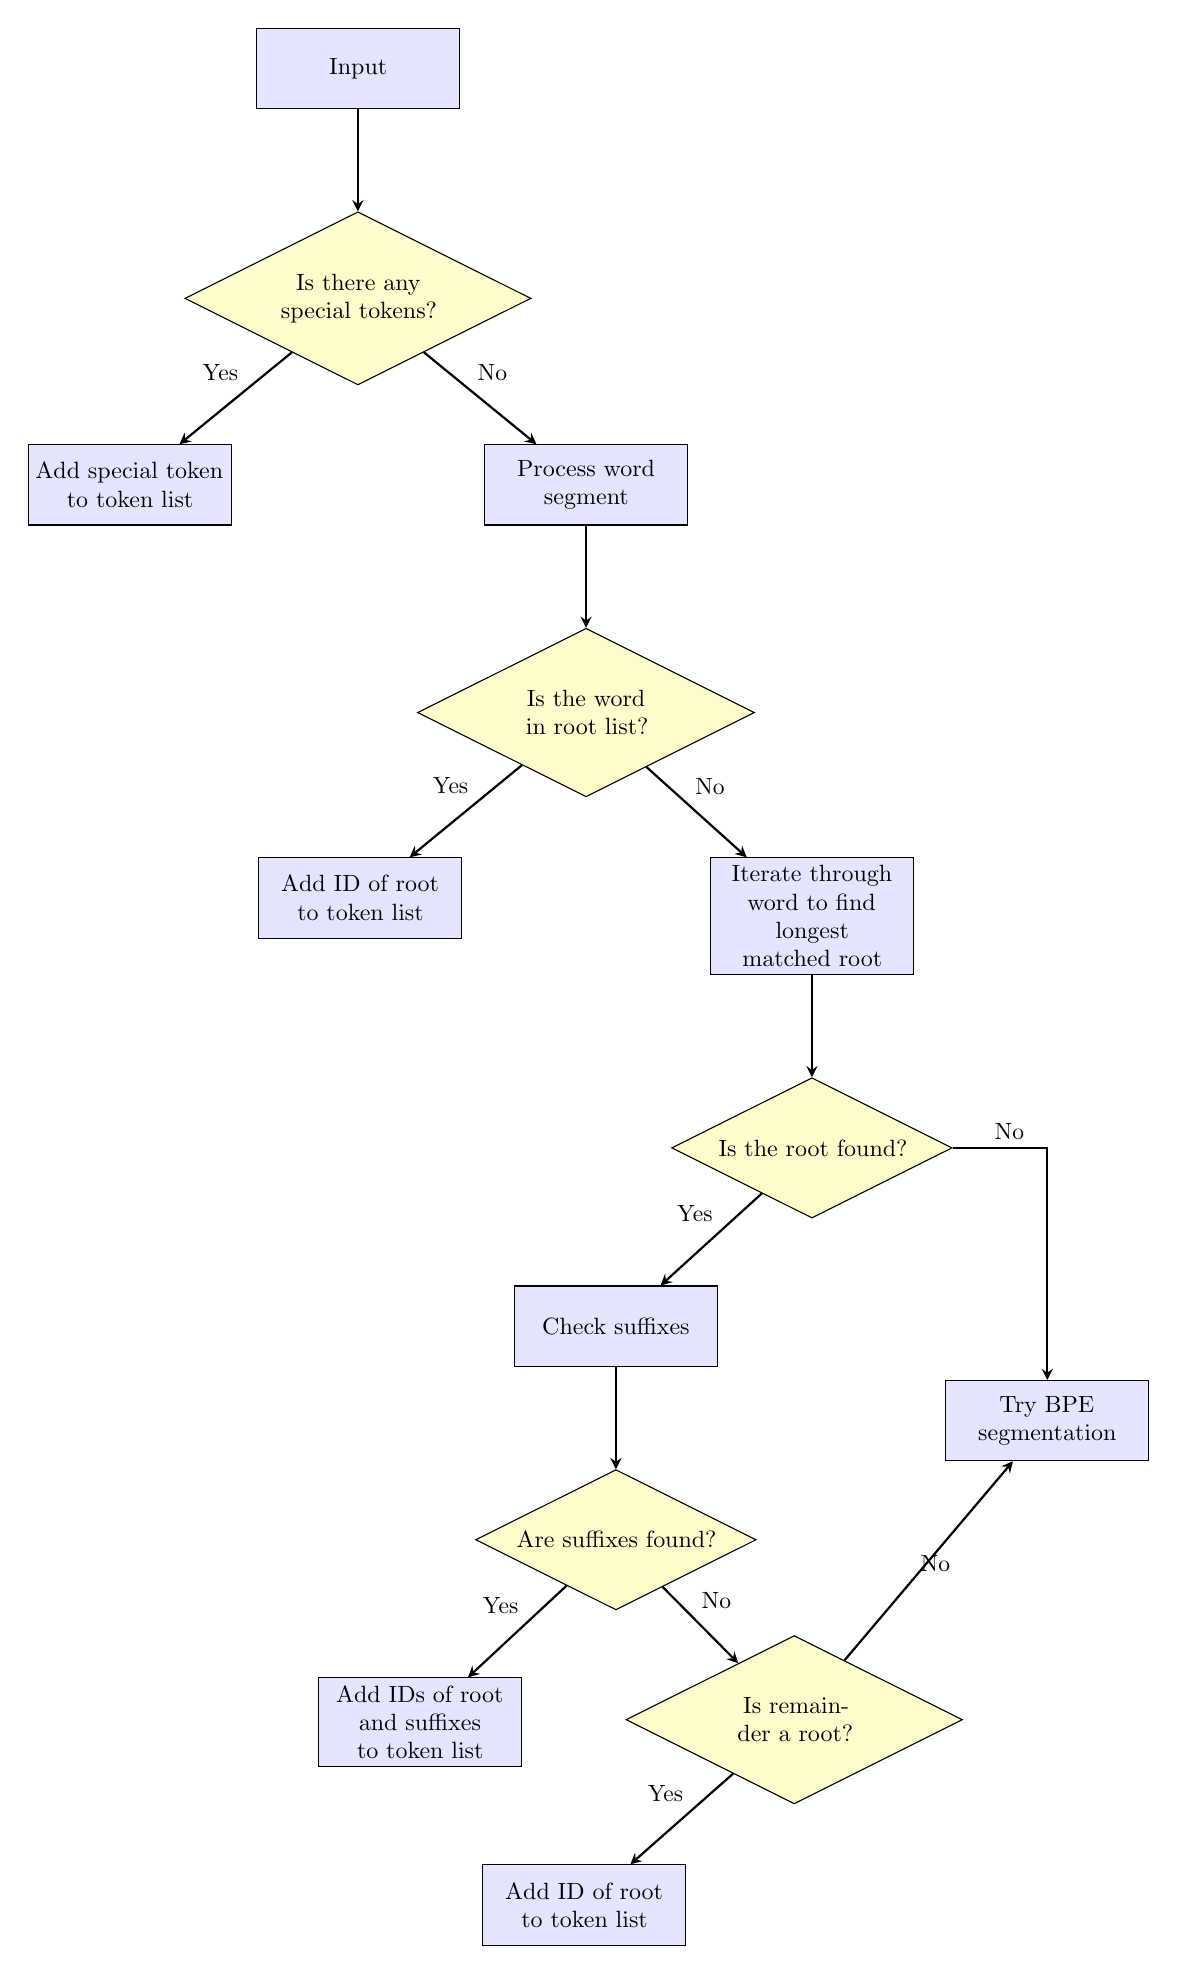
\begin{tikzpicture}[node distance=1.3cm and 1.2cm, every node/.style={transform shape, scale=0.85}]

\tikzstyle{process} = [rectangle, minimum width=2.8cm, text width=2.8cm, minimum height=1.2cm, text centered, draw=black, fill=blue!10]
\tikzstyle{decision} = [diamond, aspect=2, text width=3cm, text centered, draw=black, fill=yellow!20]
\tikzstyle{arrow} = [thick,->,>=stealth]

% Nodes
\node[process] (input_node) {Input};
\node[decision, below=of input_node] (special_check) {Is there any special tokens?};
\node[process, below left=1.3cm and 0.5cm of special_check] (add_special) {Add special token to token list};
\node[process, below right=1.3cm and 0.5cm of special_check] (process_word) {Process word segment};
\node[decision, below=1.3cm of process_word] (root_check) {Is the word in root list?};
\node[process, below left=1.3cm and 0.5cm of root_check] (add_root_id) {Add ID of root to token list};
\node[process, below right=1.3cm and 0.5cm of root_check] (iterate_root) {Iterate through word to find longest matched root};
\node[decision, below=1.3cm of iterate_root] (root_found_check) {Is the root found?};
\node[process, below left=1.3cm and 0.3cm of root_found_check] (check_suffixes) {Check suffixes};
\node[process, below right=2.5cm and 0.8cm of root_found_check] (try_bpe) {Try BPE segmentation};
\node[decision, below=1.3cm of check_suffixes] (suffixes_found_check) {Are suffixes found?};
\node[process, below left=1.3cm and 0.3cm of suffixes_found_check] (add_root_suffix_ids) {Add IDs of root and suffixes to token list};
\node[decision, below right=1.3cm and 0.3cm of suffixes_found_check] (remainder_root_check) {Is remainder a root?};
\node[process, below left=1.3cm and 0.3cm of remainder_root_check] (add_root_id_rem) {Add ID of root to token list};

% Arrows
\draw[arrow] (input_node) -- (special_check);
\draw[arrow] (special_check) -- node[above left, pos=0.4] {Yes} (add_special);
\draw[arrow] (special_check) -- node[above right, pos=0.4] {No} (process_word);
\draw[arrow] (process_word) -- (root_check);
\draw[arrow] (root_check) -- node[above left, pos=0.4] {Yes} (add_root_id);
\draw[arrow] (root_check) -- node[above right, pos=0.4] {No} (iterate_root);
\draw[arrow] (iterate_root) -- (root_found_check);
\draw[arrow] (root_found_check) -- node[above left, pos=0.4] {Yes} (check_suffixes);
\draw[arrow] (root_found_check.east) -| node[above, pos=0.3] {No} (try_bpe.north);
\draw[arrow] (check_suffixes) -- (suffixes_found_check);
\draw[arrow] (suffixes_found_check) -- node[above left, pos=0.4] {Yes} (add_root_suffix_ids);
\draw[arrow] (suffixes_found_check) -- node[above right, pos=0.4] {No} (remainder_root_check);
\draw[arrow] (remainder_root_check) -- node[above left, pos=0.4] {Yes} (add_root_id_rem);
\draw[arrow] (remainder_root_check) -- node[above right, pos=0.4] {No} (try_bpe);

\end{tikzpicture}%
}
\caption{Tokenization decision flow with root, suffix, and fallback segmentation logic.}
\end{figure}

The tokenizer is implemented in both Python and Rust, each optimized for different use cases. The Python implementation provides flexibility and ease of integration into NLP pipelines, whereas the Rust implementation prioritizes performance through parallel processing and efficient memory management. The tokenization process follows a structured pipeline consisting of three key components: dictionary-based morphological segmentation, BPE integration for subword tokenization, and the inclusion of special tokens to preserve linguistic and formatting information.

Morphological segmentation is a key component of the proposed approach, leveraging a dual-dictionary system to accurately identify and segment words. The root dictionary is constructed from high-frequency words extracted from large-scale Turkish corpora, ensuring that only base word forms are included. This dictionary is augmented with phonological normalization techniques to prevent vocabulary expansion due to phonological alternations such as final devoicing (\textit{kitap} $\rightarrow$ \textit{kitabı}), haplology (\textit{alın} $\rightarrow$ \textit{alnı}), and vowel hiatus (\textit{oyna} + \textit{yor} $\rightarrow$ \textit{oynuyor}). Furthermore, frequently used compound words such as "akarsu" and "çamaşırhane" are assigned unique identifiers to ensure they are treated as single tokens rather than being arbitrarily segmented.

The affix dictionary consists of approximately 230 linguistic elements, including suffixes, prepositions, and conjunctions. To improve efficiency and reduce redundancy, affixes with identical grammatical functions, such as the plural markers "-lAr" or the ablative markers "-dAn," are assigned a common identifier. This approach ensures that morphologically equivalent structures do not inflate the vocabulary size while preserving their grammatical roles in sentence construction.

To ensure comprehensive token coverage, the framework integrates Byte Pair Encoding (BPE) to segment words that are not explicitly listed in the morphological dictionaries. The training data for BPE was sourced from large-scale Turkish corpora, specifically \textit{umarigan/turkish\_corpus\_small} and \textit{kadirnar/combined-turkish-datasets-v4}, with a combined size of 8.52 GB. Using the SentencePiece library, a vocabulary of 10,000 subword units was generated and subsequently incorporated into the tokenizer. This enables the system to process novel words while retaining consistency in morphological decomposition.

Special tokens are introduced to handle whitespace, punctuation, capitalization, and unknown words, enhancing the tokenizer's ability to preserve linguistic structure. A dedicated token for whitespace ensures that spacing information is explicitly encoded, preserving sentence structure during tokenization. Additionally, an uppercase token is introduced to differentiate capitalized words from their lowercase counterparts without inflating the vocabulary. Additional tokens account for newline characters, tab spaces, and unknown words, preventing tokenization errors when encountering unfamiliar input.

The encoding process begins with morphological analysis, where the longest matching root is identified from the dictionary. Once the root is determined, suffix segmentation is performed by iteratively checking for affix matches. If a valid segmentation cannot be identified using the morphological dictionary, the remaining portion of the word is processed using BPE-based subword segmentation. Words that do not match any predefined root, suffix, or subword are assigned an unknown token, ensuring robustness in handling OOV terms.

The decoding process reconstructs tokenized text while adhering to linguistic rules. A reverse mapping mechanism ensures that phonological alternations are restored correctly, preserving morphosyntactic dependencies. Disambiguation rules are applied to select the most probable reconstruction based on phonetic context and grammatical constraints. This process enhances readability while maintaining fidelity to the original text.

The proposed framework provides a balance between linguistic integrity and computational efficiency. By integrating morphological analysis with BPE-based segmentation, the tokenizer achieves improved performance in capturing linguistic structures while maintaining flexibility for unseen words. Furthermore, the methodology is adaptable to other morphologically complex languages, demonstrating its potential for multilingual applications.

The construction of the tokenizer dictionary follows a structured approach that ensures comprehensive coverage of Turkish morphology while maintaining efficiency. The dictionary consists of three primary components: a root word list, an affix list, and a set of functional words such as prepositions and conjunctions. These elements form the basis of the tokenization process, enabling accurate segmentation and linguistic representation.

The root dictionary is built from a dataset of high-frequency Turkish words extracted from large-scale corpora. This dataset includes approximately 22,000 roots, ensuring broad lexical coverage. Each root is assigned a unique identifier, allowing for consistent referencing throughout the tokenization process. To improve efficiency, roots are categorized based on their length, enabling a hierarchical lookup mechanism that prioritizes longer roots before shorter alternatives. This method significantly enhances root detection speed by reducing the number of comparisons required.

An additional layer of processing is applied to handle phonological alternations in root words, which frequently occur in Turkish due to sound changes triggered by suffixation. To ensure consistency and reduce vocabulary sparsity, different phonetic realizations of the same morphological root are mapped to a single identifier. For example, final devoicing results in surface variations such as \textit{kitap} (‘book’) and \textit{kitabı} (‘its book’), both of which are assigned the same root ID. Similarly, haplology in forms like \textit{alın} (‘forehead’) and \textit{alnı} (‘his/her forehead’), and vowel hiatus in forms like \textit{oyna} + \textit{yor} $\rightarrow$ \textit{oynuyor} (‘he/she/it is playing’) are normalized through unified token mappings. This phonological normalization preserves morphological coherence while avoiding unnecessary token duplication.

In addition to root words, the dictionary includes a comprehensive inventory of approximately 230 suffixes, prepositions, and conjunctions, compiled from authoritative linguistic sources and organized according to grammatical function. To further optimize vocabulary size without compromising syntactic accuracy, affixes that perform the same grammatical role are assigned a shared identifier. For instance, plural suffixes such as \textit{-lAr}, or ablative markers like \textit{-dAn}, \textit{-tAn}, functionally represent the same morphemes but differ based on phonological context. This strategy is also applied to locative markers like \textit{-dA} and \textit{-tA}, which exhibit surface variation due to consonant alternation rules. By merging such phonologically conditioned allomorphs, the tokenizer reduces redundancy while maintaining linguistic fidelity.

Compound words represent another important aspect of Turkish morphology, wherein multiple roots combine to form a single semantic unit. To prevent incorrect segmentation, frequently used compounds such as \textit{akarsu} (‘stream’) and \textit{çamaşırhane} (‘laundromat’) are directly included in the dictionary and assigned unique token IDs. This ensures that compound expressions are treated as indivisible lexical items, preserving their semantic integrity and avoiding erroneous decomposition into root-affix pairs.

Beyond roots and affixes, the dictionary incorporates functional words such as prepositions and conjunctions, which play a crucial role in sentence structure. These elements are often challenging to tokenize correctly due to their small size and high frequency. By including them explicitly in the dictionary, the tokenizer avoids erroneous segmentations that might result from statistical subword approaches.

The integration of Byte Pair Encoding (BPE) further enhances tokenization flexibility. While the dictionary provides structured linguistic segmentation, BPE ensures robust handling of words not explicitly covered in the predefined lexicon. The BPE model is trained on a diverse Turkish corpus, incorporating approximately 10,000 subword units to supplement dictionary-based tokenization. The combined approach enables the tokenizer to efficiently process both frequent and rare words, ensuring comprehensive text coverage.

Another important aspect of the proposed framework is its ability to handle case sensitivity without increasing vocabulary size. A dedicated uppercase token is introduced to mark words that were originally capitalized. This avoids the need to store separate tokens for capitalized and lowercase versions of the same word, optimizing storage efficiency while preserving orthographic distinctions.

The dictionary-driven approach provides a balance between linguistic accuracy and computational efficiency. By leveraging structured linguistic resources, normalizing phonological variations, and integrating statistical subword segmentation, the tokenizer achieves robust performance across diverse text types. The next section will describe the encoding and decoding processes in detail, outlining how tokenization is applied in practice to segment and reconstruct text.

The encoding process follows a hierarchical approach that ensures linguistic consistency while maintaining computational efficiency. The tokenizer operates in a multi-step pipeline that sequentially applies morphological analysis, affix segmentation, and subword processing. This structured approach optimizes tokenization accuracy while preserving essential linguistic features.

The encoding process begins with preprocessing, where special characters and formatting elements are replaced with predefined tokens. Whitespace characters such as spaces, newlines, and tab spaces are explicitly encoded using dedicated tokens. This step ensures that text formatting is preserved, preventing information loss in structured text. Additionally, words that begin with capital letters are marked with an uppercase token to maintain case information without inflating the vocabulary.

Following preprocessing, the tokenizer applies root detection using a hierarchical lookup strategy. The algorithm first searches for the longest matching root in the dictionary, prioritizing exact matches before considering phonological variants. If a match is found, the root is assigned its corresponding token ID. In cases where no direct match is identified, alternative scenarios such as compound words or phonologically altered roots are considered. This flexible approach ensures that words are correctly segmented even when phonological modifications are present.

Once the root is identified, suffix segmentation is performed iteratively. The algorithm checks for affix matches in the suffix dictionary and assigns token IDs accordingly. Each identified suffix is treated as a separate token, maintaining its grammatical function while ensuring proper segmentation. The suffix matching process continues until no further valid suffixes can be extracted. If an affix is ambiguous or overlaps with multiple possible segmentations, a probabilistic model selects the most likely segmentation based on corpus frequency data.

If a word does not match any predefined root or suffix, Byte Pair Encoding (BPE) is applied as a fallback mechanism. The BPE model segments the word into subword units based on a pre-trained vocabulary, ensuring that unknown words are processed effectively. This hybrid approach prevents the tokenizer from failing on unseen words while maintaining the linguistic integrity of known structures.

For example, the word \textit{kalktığımızda} (‘when we stood up’) is segmented into its root and affix components as follows:

\textbf{Input text:} \texttt{"Kalktığımızda hep birlikte yürüdük."} (“When we stood up, we walked together.”)

\textbf{Token sequence:} \texttt{[uppercase], kalk, tığ, ımız, da, [space], hep, [space], birlikte, [space], yürü, dü, k, .}

\textbf{Token IDs:} \texttt{0, 1502, 22280, 22285, 22278, 1, 2300, 1, 4803, 1, 2280, 22296, 22617, 22582}

\begin{figure}[htbp]
\centering
\resizebox{\textwidth}{!}{%
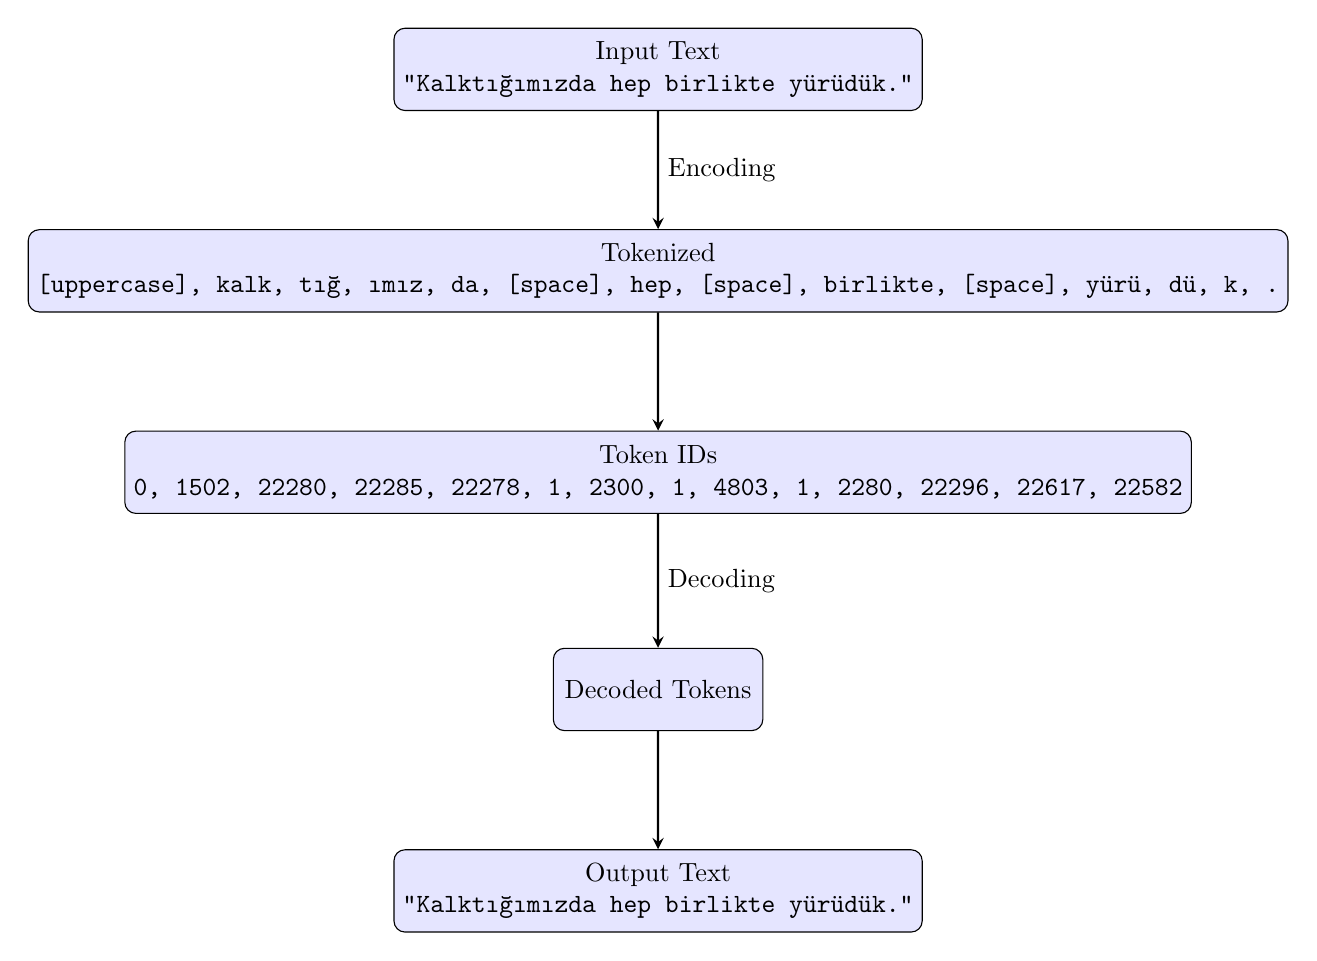
\begin{tikzpicture}[node distance=1.5cm and 0.7cm, every node/.style={transform shape, scale=0.95}]
\tikzset{
  mystep/.style={
    rectangle, rounded corners, draw=black, fill=blue!10,
    minimum height=1.1cm, minimum width=2.8cm,
    text centered, align=center
  },
  arrow/.style={->, thick, >=stealth}
}

\node[mystep] (text) {Input Text \\ \texttt{"Kalktığımızda hep birlikte yürüdük."}};
\node[mystep, below=of text] (tokenized) {Tokenized \\ \texttt{[uppercase], kalk, tığ, ımız, da, [space], hep, [space], birlikte, [space], yürü, dü, k, .}};
\node[mystep, below=of tokenized] (ids) {Token IDs \\ \texttt{0, 1502, 22280, 22285, 22278, 1, 2300, 1, 4803, 1, 2280, 22296, 22617, 22582}};
\node[mystep, below=1.7cm of ids] (reconstruct) {Decoded Tokens};
\node[mystep, below=of reconstruct] (finaltext) {Output Text \\ \texttt{"Kalktığımızda hep birlikte yürüdük."}};

\draw[arrow] (text) -- (tokenized) node[midway, right] {Encoding};
\draw[arrow] (tokenized) -- (ids);
\draw[arrow] (ids) -- (reconstruct) node[midway, right] {Decoding};
\draw[arrow] (reconstruct) -- (finaltext);

\end{tikzpicture}%
}
\caption{Encoding and decoding process for the sentence “Kalktığımızda hep birlikte yürüdük.”}
\end{figure}

This example demonstrates how the encoder accurately identifies the root \textit{kalk} (“stand up”), segments its suffixes (\textit{-tığ} “past nominalizer”, \textit{-ımız} “our”, \textit{-da} “when/at”), and preserves syntactic structure using dedicated space and punctuation tokens. Each token corresponds to a morphologically meaningful unit, enabling interpretable and reversible text representations.

The decoding process reconstructs surface text from tokenized sequences while maintaining linguistic accuracy. Token IDs are mapped back to their textual forms, and affixes are recombined according to their grammatical function. During this step, phonological alternations are reversed: rules for soft consonantization, vowel deletion, and contraction are reapplied to ensure natural word formation.

Capitalization is restored using a dedicated \texttt{[uppercase]} token, which automatically capitalizes the first letter of the following word. Space and punctuation tokens (\texttt{[space]}, \texttt{.}, etc.) are replaced with their respective characters, maintaining sentence layout. If an unknown or out-of-vocabulary token is encountered, a placeholder is inserted to allow for post-processing or human review.

Consider another example:

\textbf{Token sequence:} \texttt{[uppercase], kitap, [space], okuma, yı, [space], sev, i, yor, um, .}

\textbf{Decoded output:} \texttt{"Kitap okumayı seviyorum."} (“I like reading books.”)

This process demonstrates how the tokenizer ensures both accuracy and efficiency in text reconstruction, preserving morphological structure while maintaining fluency.

The proposed framework successfully integrates morphological analysis with subword segmentation, creating a robust tokenizer optimized for morphologically complex languages. By balancing linguistic integrity and computational efficiency, this approach offers a scalable solution adaptable to multiple languages. Future work may explore extending this framework to other agglutinative languages, optimizing it for real-time applications, and integrating additional linguistic features for enhanced performance.

\section{Results and Analysis}
\label{sec:results}

The performance of the proposed morphological tokenizer was evaluated using the TR-MMLU benchmark dataset, which comprises over 1.6 million characters and approximately 200,000 words curated specifically for Turkish \cite{bayram_setting_2025}. This dataset is designed to reflect the linguistic complexity of Turkish, including its rich morphology, agglutinative structures, and diverse syntactic constructions. As such, it provides a rigorous basis for assessing tokenization quality in morphologically complex languages.

The evaluation compared five different tokenizers: \texttt{google/gemma-2-9b}, \texttt{meta-llama/Llama-3.2-3B}, \texttt{Qwen/Qwen2.5-7B-Instruct}, \texttt{CohereForAI/aya-expanse-8b}, and the proposed \texttt{turkish\_tokenizer}. Each tokenizer was assessed using a consistent set of linguistic and computational metrics introduced in \cite{bayram_tokenization_2025}. These metrics include total token count, vocabulary size, number of unique tokens, Turkish Token Percentage (TR~\%), and Pure Token Percentage (Pure~\%). TR~\% quantifies the proportion of tokens that correspond to valid Turkish words or morphemes, while Pure~\% measures the proportion of tokens that fully align with unambiguous root or affix boundaries, thus reflecting morphological integrity.

\begin{table}[h]
\centering
\caption{Performance of the proposed \texttt{turkish\_tokenizer} on the TR-MMLU dataset.}
\label{tab:turkish_tokenizer_results}
\begin{tabular}{|l|c|}
\hline
\rowcolor[HTML]{DDDDDD} 
\textbf{Metric} & \textbf{Value} \\ \hline
Vocabulary Size & 32,768 \\ \hline
Total Token Count & 707,727 \\ \hline
Processing Time (s) & 0.6714 \\ \hline
Unique Token Count & 11,144 \\ \hline
Turkish Token Count & 10,062 \\ \hline
Turkish Token Percentage (TR \%) & 90.29\% \\ \hline
Pure Token Count & 9,562 \\ \hline
Pure Token Percentage (Pure \%) & 85.80\% \\ \hline
\end{tabular}
\end{table}

The proposed \texttt{turkish\_tokenizer} demonstrated the highest linguistic alignment across all evaluated metrics. It achieved a TR~\% of 90.29\% and a Pure~\% of 85.80\%, substantially outperforming all competing tokenizers. In comparison, \texttt{google/gemma-2-9b} reached a TR~\% of only 40.96\% and a Pure~\% of 28.49\%, indicating that the majority of its tokens do not represent full morphemes. Similarly, \texttt{meta-llama/Llama-3.2-3B} produced a TR~\% of 45.77\% and a Pure~\% of 31.45\%, while \texttt{Qwen2.5} and \texttt{aya-expanse} achieved TR~\% values of 40.39\% and 53.48\%, respectively.

Despite employing significantly smaller vocabulary sizes, the proposed tokenizer demonstrated better linguistic segmentation. With a vocabulary of 32,768 tokens and 11,144 unique tokens used during evaluation, it balanced generalization and expressiveness more effectively than models such as \texttt{gemma-2-9b} and \texttt{aya-expanse}, which rely on vocabularies of over 255,000 tokens. These large-vocabulary tokenizers, rooted in frequency-based subword segmentation, tend to fragment morphologically rich expressions and introduce ambiguity in downstream tasks. In contrast, the morphological awareness of the \texttt{turkish\_tokenizer} enables semantically coherent token formation and more consistent syntactic parsing.

Although the total token count generated by the proposed tokenizer (707,727) exceeds those of the other models—for instance, \texttt{aya-expanse} produced 434,526 tokens—this increase is offset by gains in interpretability and linguistic fidelity. High TR~\% and Pure~\% scores suggest reduced reliance on spurious subword splits and improved preservation of morphosyntactic structure. This is particularly beneficial for tasks such as syntactic parsing, translation, summarization, and question answering, where semantic consistency across tokens is essential.

These findings support the hypothesis introduced in \cite{bayram_tokenization_2025}, which argues that high linguistic alignment in tokenization correlates strongly with downstream model performance in morphologically rich and low-resource languages. While conventional subword tokenizers may suffice for high-resource languages like English, they exhibit clear limitations in Turkish unless informed by morphological structure. The results presented here highlight the effectiveness of combining rule-based linguistic analysis with subword strategies to produce tokenizers that are both accurate and efficient in morphologically complex settings.

To illustrate the linguistic fidelity of different tokenization strategies, we present a qualitative comparison using the Turkish sentence:

\textit{"Atasözleri geçmişten günümüze kadar ulaşan anlamı bakımından mecazlı bir mana kazanan kalıplaşmış sözlerdir."} \\
(“Proverbs are fixed expressions passed down from the past to the present that acquire a metaphorical meaning in terms of their significance.”)

This sentence contains a wide range of morphological features, including compound words, multiple derivational and inflectional suffixes, and root forms that undergo phonological alternations. These properties make it an ideal test case for evaluating the morphological sensitivity of different tokenizers.

\vspace{1em}

\textbf{Proposed Hybrid Tokenizer:} \\
The hybrid morphological tokenizer segments the sentence into linguistically meaningful units with high fidelity. It produces: \\
\texttt{["<uppercase>", "atasöz", "ler", "i", "<space>", "geçmiş", "ten", "<space>", "gün", "üm", "üz", "e", "<space>", "kadar", "<space>", "ulaş", "an", "<space>", "anlam", "ı", "<space>", "bakım", "ın", "dan", "<space>", "mecaz", "lı", "<space>", "bir", "<space>", "mana", "<space>", "kazan", "an", "<space>", "kalıp", "laş", "mış", "<space>", "sözle", "r", "dir", "."]} \\
It correctly separates suffixes (\texttt{"ler", "i", "ın", "dan", "lı", "an", "mış", "dir"}), extracts root forms such as \texttt{"atasöz", "gün", "mana"}, and employs special tokens like \texttt{"<uppercase>"} and \texttt{"<space>"} to preserve orthographic structure.

\vspace{1em}

\textbf{Gemma-3:} \\
The tokenizer \texttt{google/gemma-3} segments the sentence as: \\
\texttt{["<bos>", "At", "as", "öz", "leri", " geçmiş", "ten", " gün", "ümü", "ze", " kadar", " ulaş", "an", " anlam", "ı", " bakım", "ından", " mec", "az", "lı", " bir", " mana", " kaz", "anan", " kal", "ı", "pla", "ş", "mış", " söz", "lerdir", "."]} \\
Although it captures some suffixes like \texttt{"ten"} and \texttt{"ından"}, it fragments common roots (\texttt{"At", "as", "öz"} instead of \texttt{"atasöz"}) and fails to isolate inner morphemes in forms such as \texttt{"lerdir"} and \texttt{"kazanan"}, limiting morphological interpretability.

\vspace{1em}

\textbf{LLaMA-3.2:} \\
The tokenizer \texttt{meta-llama/Llama-3.2-3B} yields: \\
\texttt{["<|begin\_of\_text|>", "At", "as", "öz", "leri", " geçmiş", "ten", " gün", "ümü", "ze", " kadar", " ", "ula", "ş", "an", " anlam", "ı", " bakımından", " me", "ca", "z", "lı", " bir", " mana", " kaz", "anan", " kal", "ı", "pla", "ş", "mış", " söz", "lerdir", "."]} \\
This tokenizer combines morphologically valid segments like \texttt{"bakımından"} and \texttt{"kazanan"} with fragmented roots like \texttt{"At", "as", "öz"}, creating inconsistency in morpheme alignment.

\vspace{1em}

\textbf{Qwen2.5:} \\
The tokenizer \texttt{Qwen/Qwen2.5} outputs: \\
\texttt{["At", "as", "öz", "leri", " geçmiş", "ten", " gün", "üm", "ü", "ze", " kadar", " ulaş", "an", " anlamı", " bakım", "ından", " me", "ca", "z", "lı", " bir", " mana", " kaz", "anan", " kal", "ı", "pla", "ş", "mış", " söz", "ler", "dir", "."]} \\
While suffixes such as \texttt{"ten"} and \texttt{"ından"} are recognized, the tokenizer introduces redundant splits like \texttt{"üm", "ü", "ze"}, reducing the linguistic coherence of the token stream.

\vspace{1em}

\textbf{Aya-Expanse:} \\
The tokenizer \texttt{CohereForAI/aya-expanse} returns: \\
\texttt{["<BOS\_TOKEN>", "At", "as", "öz", "leri", " geçmiş", "ten", " günümüze", " kadar", " ulaşan", " anlamı", " bakımından", " mec", "az", "lı", " bir", " mana", " kazanan", " kalı", "pl", "aş", "mış", " söz", "lerdir", "."]} \\
It retains some complete word forms such as \texttt{"günümüze"} and \texttt{"ulaşan"}, but still fragments compounds like \texttt{"kalıplaşmış"} and splits the root \texttt{"atasöz"}, reducing morphological traceability.

\vspace{1em}

\textbf{Phi-4:} \\
The tokenizer \texttt{microsoft/phi-4} produces: \\
\texttt{["At", "as", "ö", "z", "leri", " geç", "mi", "ş", "ten", " gün", "üm", "ü", "ze", " kadar", " ", "ula", "ş", "an", " an", "lam", "ı", " bak", "ım", "ından", " me", "ca", "z", "lı", " bir", " mana", " kaz", "anan", " kal", "ı", "pla", "ş", "m", "ış", " sö", "z", "ler", "dir", "."]} \\
This tokenizer over-fragments even basic stems like \texttt{"geçmiş"} into \texttt{"geç", "mi", "ş"} and \texttt{"anlam"} into \texttt{"an", "lam"}, increasing token count and reducing interpretability.

\vspace{1em}

\textbf{YTU Turkish GPT-2:} \\
The tokenizer \texttt{ytu-ce-cosmos/turkish-gpt2-large-750m-instruct-v0.1}, trained on Turkish corpora, yields: \\
\texttt{["At", "as", "öz", "leri", " geçmişten", " günümüze", " kadar", " ulaşan", " anlamı", " bakımından", " mec", "az", "lı", " bir", " mana", " kazanan", " kalıp", "laşmış", " söz", "lerdir", "."]} \\
Although it still segments \texttt{"atasözleri"} incorrectly, it performs well with forms like \texttt{"geçmişten"}, \texttt{"günümüze"}, and \texttt{"bakımından"}, showing the advantage of Turkish-specific pretraining.

\vspace{1em}

\textbf{GPT-4o:} \\
The tokenizer \texttt{gpt-4o-o200k\_base} generates: \\
\texttt{["At", "as", "öz", "leri", " geçmiş", "ten", " gün", "ümü", "ze", " kadar", " ulaş", "an", " anlam", "ı", " bakım", "ından", " mec", "az", "lı", " bir", " mana", " kaz", "anan", " kal", "ı", "pla", "ş", "mış", " söz", "ler", "dir", "."]} \\
Its segmentation strategy is similar to LLaMA and Qwen—partially aware of Turkish morphemes but limited by frequent over-segmentation of compound and derived forms.

\vspace{1em}

The results presented in this section provide strong empirical support for the hypothesis introduced in the introduction: tokenizers that explicitly incorporate morphological and phonological knowledge of Turkish can outperform general-purpose models in both segmentation accuracy and linguistic coherence. While most state-of-the-art tokenizers struggle with root-fragmentation, over-segmentation, and inconsistent affix treatment, the proposed hybrid tokenizer consistently identifies morpheme boundaries, preserves semantically meaningful units, and reduces vocabulary redundancy. These findings validate the motivation behind this work: morphologically informed tokenization is essential for robust and interpretable NLP in agglutinative languages like Turkish. The qualitative comparisons presented here illustrate not only the performance gap between general and language-specific tokenizers, but also the need for tokenizer architectures that respect language-internal rules.

\section{Conclusion}
\label{sec:conclusion}

In this study, we introduced a linguistically-informed hybrid tokenization framework specifically designed to address the challenges posed by morphologically rich and low-resource languages, with Turkish serving as the primary case study. By integrating rule-based morphological analysis with subword segmentation techniques such as Byte Pair Encoding (BPE), our approach seeks to preserve morpheme boundaries, minimize vocabulary redundancy, and improve syntactic and semantic coherence during tokenization.

Empirical evaluations on the TR-MMLU dataset demonstrated that the proposed \texttt{turkish\_tokenizer} significantly outperforms existing state-of-the-art tokenizers—including \texttt{gemma-2}, \texttt{llama-3}, \texttt{qwen2.5}, and \texttt{aya-expanse}—in both Turkish Token Percentage (TR~\%) and Pure Token Percentage (Pure~\%), achieving 90.29\% and 85.80\%, respectively. These metrics reflect the tokenizer’s strong alignment with the linguistic structure of Turkish, a crucial factor for downstream NLP tasks. The tokenizer also exhibited efficient vocabulary utilization with only 32,768 entries and showed robust performance in handling morphosyntactic structures across diverse sentence types.

Qualitative analyses further reinforced the superiority of our approach, revealing that the proposed tokenizer segments text into linguistically meaningful units and accurately preserves suffixes, compound forms, and phonologically altered variants—challenges frequently mishandled by general-purpose, frequency-driven tokenization strategies. The findings presented here reaffirm the thesis proposed in \cite{bayram_tokenization_2025}, namely that tokenization strategies rooted in linguistic structure are not only desirable but necessary for accurate and efficient language modeling in morphologically complex settings. As NLP continues to evolve toward inclusive, multilingual systems, the development of linguistically aware tokenization methods will be critical for ensuring equity in language technologies.

Future directions include extending this hybrid framework to other agglutinative and typologically diverse languages, refining the morphological rules through semi-supervised learning, and exploring integration with multilingual LLM pretraining pipelines to optimize performance in low-resource language environments.

\bibliographystyle{unsrt}
\bibliography{tokenizer}

\end{document}
